\documentclass[12pt,twoside,a4paper]{article}
\usepackage[margin=2cm]{geometry}
\usepackage{xspace,amsmath,amssymb,graphicx,color,paralist,upquote,textcomp}
\usepackage[small]{caption}
\usepackage[colorlinks=true,citecolor=darkblue,linkcolor=darkblue,
urlcolor=darkblue]{hyperref} \usepackage{bookmark}
\protect{\renewcommand{\arraystretch}{1.2}}
\pagestyle{myheadings}
\pagenumbering{arabic}
\protect{\setcounter{page}{1}}
\raggedbottom
\tolerance=10000
\setlength{\parskip}{0.5em}

\definecolor{Mygrey}{gray}{0.975}
\definecolor{darkblue}{rgb}{0.0,0.0,0.55}

%% Margin references to books
\newcommand{\MD}[1]{\marginpar{\raggedright\bf MD\ #1}}
\newcommand{\DA}[1]{\marginpar{\raggedright\bf DA\ #1}}
\newcommand{\PP}[1]{\marginpar{\raggedright\bf P\ #1}}
\newcommand{\TS}[1]{\marginpar{\raggedright\bf TS\ #1}}
\newcommand{\EH}[1]{\marginpar{\raggedright\bf EH\ #1}}

%% Grey boxes and other shortcuts.
\newcommand{\bx}[1]{\noindent\fcolorbox{black}{Mygrey}{\parbox{\textwidth}{#1}}\\[-1mm]}
\newcommand{\bxc}[1]{\noindent\fcolorbox{black}{Mygrey}{\parbox{\textwidth}{\centering{}#1}}\\[-1mm]}
\newcommand{\bqx}[1]{\noindent\fcolorbox{black}{Mygrey}{\parbox[t]{15cm}{#1}}\\[-2mm]}
\newcommand{\Eref}[1]{Equation~(\ref{eq:#1})}
\newcommand{\eref}[1]{equation~(\ref{eq:#1})}
\newcommand{\Sec}[1]{Section~\ref{sec:#1}}
\newcommand{\question}{\noindent\textbf{Question:}\xspace}
\newcommand{\labtitle}[2]{\begin{center}\Huge{Laboratory #1}\\\Large{#2}\end{center}}

%% Matlab
\newcommand{\Mlab}{\textsc{Matlab}\xspace}
\newcommand{\Minput}[1]{\newline\indent\indent\texttt{>> #1}}
\newcommand{\Matlab}[3]{\\[2mm]\indent\indent\begin{minipage}{12cm}{
        \setlength{\parindent}{5mm}
        \noindent\texttt{>> #1}\nopagebreak[4]\\
        \noindent\texttt{#2 = }\nopagebreak[4]\\[2mm]
        \indent\indent\parbox{5cm}{\texttt{#3}}}\end{minipage}\\[2mm]}
\newcommand{\Moutput}[2]{\newline\indent\indent\texttt{#1 = }\newline
        \indent\indent\indent\indent\texttt{#2}\newline}
\newcommand{\qu}{\textquotesingle}

%% Math
\newcommand{\bv}[1]{\mbox{{\bf #1}}}
\newcommand{\Grad}{\mbox{\boldmath $\nabla$}}
\newcommand{\Div}{\Grad\!\cdot}
\newcommand{\Curl}{\Grad\!\times}
\newcommand{\delsq}{\nabla^2}
\newcommand{\mean}[1]{\left\langle{#1}\right\rangle}
\newcommand{\infd}{\textrm{d}}
\newcommand{\diff}[2]{\frac{\infd #1}{\infd #2}}
\newcommand{\difftwo}[2]{\frac{\infd^2 {#1}}{\infd {#2}^2}}
\newcommand{\pdiff}[2]{\frac{\partial #1}{\partial #2}}
\newcommand{\pdiffcon}[3]{\left(\frac{\partial #1}{\partial #2}\right)_{#3}}
\newcommand{\pdifftwo}[2]{\frac{\partial^2 {#1}}{\partial {#2}^2}}
\newcommand{\pdifftwomix}[3]{\frac{\partial^2 {#1}}{\partial {#2}\,\partial {#3}}}
\newcommand{\vel}{\bv{v}}
\newcommand{\expu}[1]{\textrm{e}^{#1}}
\newcommand{\ehat}{\bv{e}}

\renewcommand{\thefootnote}{\fnsymbol{footnote}}

% make autoref references nicer
\makeatletter
\def\tagform@#1{\maketag@@@{\ignorespaces#1\unskip\@@italiccorr}}
\let\orgtheequation\theequation
\def\theequation{(\orgtheequation)}
\makeatother \newcommand{\runtitle}{DTP --- Fourier analysis}
\markboth{\runtitle{}}{\runtitle{}}

\title{DTP practise problems:\\ Fourier analysis of time-series and
  functions} \author{Prof.~Richard Katz}

\begin{document}

\maketitle{}

Data-files and functions used in this lab can be found at
\begin{center}
  \url{http://www.earth.ox.ac.uk/~richardk/teaching/DTP/fourier/}
\end{center}

\subsection*{Matlab notes: loops}

In programming, it is often useful to have the program do the same
task repeatedly.  Instead of writing a long, repetitive list of
instructions in your program, you can use a \textit{loop}.  A loop is
a program element that tells the computer to execute a block of code
repeatedly, until some stopping-criterion is satisfied.  The simplest
type of loop is a \textit{for-loop}.  This type says: ``for each
number in this list of numbers, execute the enclosed block of code.''
After the program executes the code for the last entry, it stops
looping and moves along.

Here's a simple example
\begin{verbatim}
    for i=1:3
       vec(i) = 10 + i
    end
\end{verbatim}
which will produce a vector with entries 11, 12, 13. The line(s)
between the \texttt{for} statement and the \texttt{end} statement are
the code that gets executed repeatedly.

Here's a more relevant example:
\begin{verbatim}
    x = linspace(-5,5,10000);
    y = zeros(size(x));
    for j=1:2:7
       y = y + sin(2*pi*j*x/10); % Note the use of the loop index, j
       plot(x,y,'-k'); 
       title(['Series sum at j = ',num2str(j)]); xlabel('x'); ylabel('y');
       pause;                    % wait for key-press by user
    end
\end{verbatim}
Note that the loop index \texttt{j} is incremented by 2 each time the
enclosed code is executed.  See \texttt{help for} for more
information.

\Mlab also provides a \texttt{while} loop.  See \texttt{help while}
for details.

\section{Fourier series}

\begin{enumerate}
\item Prove the orthogonality relationship given in lecture
  \begin{displaymath}
    \int_{t_0}^{t_0+T}\cos\left(\frac{2\pi r}{T}t\right)
    \cos\left(\frac{2\pi s}{T}t\right)\,\infd t=
    \begin{cases}
      T/2 & \text{for $r=s$} \\
      0 & \text{for $r\ne s$}
    \end{cases}.
  \end{displaymath}
  Hint: use the trigonometric identity
  $$\cos a\cos b = \frac{\cos(a - b) + \cos(a+b)}{2}.$$
\item For this problem, $f(x) = x$ in the range $-\pi<x\le\pi$, and
  $f(x+2\pi) = f(x)$.
  \begin{enumerate}
  \item Use \Mlab to plot the function $f$ in the range from $-2\pi$
    to $2\pi$.
  \item Find the Fourier series of the function $f$.
  \item Use your result to show that
    $$1 - \frac{1}{3} + \frac{1}{5} - \frac{1}{7} + ... =
    \frac{\pi}{4}.$$ (\textit{Hint: try evaluating the series at
      $x=\pi/4$ and $\pi/2$.})
  \item Use \Mlab to create plots of your series on top of the
    function $f$ for the first 1, 3, and 20 terms in the series.
  \end{enumerate}
\item For this problem, the function $f$ is given by the following
  plot.
  \begin{center}
    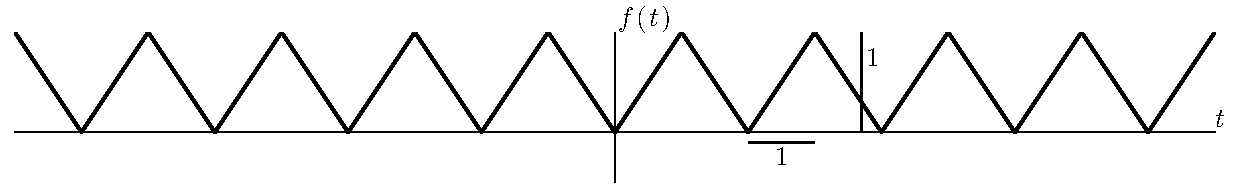
\includegraphics[width=6in]{../figs/L14/JaggedFunction}
  \end{center}
  \begin{enumerate}
  \item State the period $T$.
  \item Write a mathematical representation of $f(t)$.
  \item Is $f$ even, odd, or neither?
  \item Calculate the Fourier series of $f$.
  \item Create plots of your answer to the previous part, on top of
    the function $f$, for a sum of the first 1, 3, and 20 terms in the
    series.
  \end{enumerate}
\end{enumerate}


\subsection*{Matlab notes: data structures}

\textit{Data structures} are simply a way to bundle together variables
of different types.  Suppose we're keeping track of the attributes of
our friends using \Mlab.  We might have a friend named Jo,
\Matlab{Jo~=~struct(\qu{}Age\qu{},19,\qu{}Col\qu{},\qu{}St.~Annes\qu{},\qu{}Sgl\qu{},1,\qu{}Mob\qu{},\qu{}07974-456789\qu{})}
{Jo}{Age:~19\\Col:~\qu{}St.~Annes\qu{}\\Sgl:~1\\Mob:~\qu{}07974-456789\qu{}}
and another friend named Sam, \Minput{Sam.Age = 20;} \Minput{Sam.Col =
  \qu{}Lincoln\qu{};} \Minput{Sam.Sgl = 0;}
\Minput{Sam.Mob = \qu{}unknown\qu{};}\\
Both of these methods are acceptable for creating structures in \Mlab.

To use the data within a structure, \Matlab{S = Sam.Age +
  Jo.Age}{S}{39}

Many \Mlab functions use structures as input or output. You can use
them in your own functions, too. Experiment on the command line to
learn more.

\section{Discrete Fourier series}


\begin{enumerate}
\item This problem asks you to create a synthetic time-series, take
  its discrete Fourier series, and then reconstruct the time-series
  from the coefficients of the discrete Fourier series.
  \begin{enumerate}
  \item Create a vector of linearly spaced times with 102 points,
    starting from zero and having a maximum of $T=5$ years. Create a
    synthetic time-series using this vector, based on the formula
    \begin{displaymath}
      y(t) = \sum_{r=1}^3 \frac{3}{r}\sin(2\pi r t/T) +
      \sum_{s=1}^3\frac{6}{s}\cos(2\pi s^2 t/T).
    \end{displaymath}
    Plot your synthetic time-series.
  \item Compute the coefficients of the discrete Fourier series using
    the function \texttt{dfs}. Examine and understand the output data
    structure. Hint: \texttt{F = dfs(y(1:end-1))}. This will ensure
    that your time-series has an odd number of points and is periodic.
  \item Write a \Mlab function called \texttt{idfs} (for
    \textit{inverse discrete Fourier series}).  Your function should
    take the output structure from \texttt{dfs} and recreate and
    output the time-series.
  \item Apply your \texttt{idfs} function to the results from part
    (b). Check your result by subtracting the original time-series
    from the reconstructed one.
  \end{enumerate}
\item For this problem we'll analyse the variations in insolation that
  arise from Milankovitch cycles. Insolation is the rate of energy
  (Watts) delivery by solar radiation at the top of the atmosphere,
  per area (m$^2$).  Milankovitch cycles are cyclical changes in the
  parameters of the Earth's orbit around the sun.

  The file InsolationJune65NData.txt contains data on the flux of
  solar energy (W/m$^2$) at 65$^\circ$ N in June (i.e.~Northern
  hemisphere summer), recorded every 1000 years. These data actually
  derive from a calculation of orbital variations that is run backward
  in time to ``hind-cast'' insolation. Inspect the file and then load
  it into \Mlab.
  \begin{enumerate}
  \item Plot the insolation record as a function of time.  What is its
    mean and standard deviation?  Describe the variations in terms of
    a percentage deviation from the mean.
  \item Use the \Mlab function \texttt{dfs} to compute the
    coefficients of the discrete Fourier series.  Create a vector of
    periods corresponding to coefficients. Plot the relative power
    (variance) spectrum as a function of period in years using a
    log-log plot (\texttt{help loglog} for information).
  \item Overlay on this plot vertical lines at the dominant periods of
    orbital variation:
    \begin{enumerate}
    \item Eccentricity (oscillation between a more circular and a more
      elliptical orbit): 100 ka.
    \item Obliquity (oscillation in the tilt of Earth's rotation
      axis): 42 ka.
    \item Precession (wobble of the Earth rotation axis): 19 and 23
      ka.
    \end{enumerate}
  \item Comment on the relative magnitude of each of these peaks (as
    well as any others that you see) in the spectrum.
  \end{enumerate}
\item For this problem, we'll again analyse the time-series from
  Lisiecki and Raymo that you worked with in Laboratory 5.  Download
  the data again, if necessary (LisieckiRaymoData.txt), and load it
  into \Mlab.
  \begin{enumerate}
  \item Interpolate the data from the previous 1 million years onto a
    regularly spaced series with time interval of 1000 years, as you
    did in problem 3b of Laboratory 5.  Ensure that your series has an
    odd number of points.
  \item Make a plot of the interpolated time-series.
  \item Use the \Mlab function \texttt{dfs} to compute the
    coefficients of the discrete Fourier series.  Plot the variance as
    a function of period (years). Label your axes appropriately.
  \item Identify the clear peaks of the variance spectrum.  What are
    their periods? How might you interpret this pattern, given what
    you know about $\delta^{18}$O? Are there similarities between this
    spectrum and the one you produced for insolation variability due
    to Milankovitch cycles?  Interpret this comparison.
  \item Repeat steps (a)--(d) for the period from 1 to 2 million years
    ago.  You may wish to use a grid spacing of 2000 years.
  \end{enumerate}
\end{enumerate}


\subsection*{Matlab notes: \texttt{fit} and \texttt{legend}}

First let's review the use of the \texttt{fit} command in \Mlab.  This
provides a simple way to fit functions to time-series data.  Suppose
that you have a time-series of data with times stored in the vector
\texttt{time} and measurements stored in the vector \texttt{vals}.
The \texttt{polyfit} command can be used as follows.  \Minput{f1 =
  polyfit(time,vals,1); \% fit a straight line} \Minput{f2 =
  polyfit(time,vals,2); \% fit a quadratic polynomial} \Minput{f3 =
  polyfit(time,vals,3); \% fit a cubic polynomial} \Minput{line\_model
  = f1(1)*time + f1(2);} \Minput{quad\_model = f2(1)*time.\^{}2 +
  f2(2)*time + f2(3);} \Minput{cube\_model = f3(1)*time.\^{}3 +
  f3(2)*time.\^{}2 + f3(3)*time + f3(4);}
\Minput{plot(time,vals,\qu{}k\qu{},time,line\_model,\qu{}r\qu{}); hold
  on;}
\Minput{plot(time,quad\_model,\qu{}b\qu{},time,cube\_model,\qu{}g\qu{});
  hold off;}
\Minput{legend(\qu{}data\qu{},\qu{}poly1\qu{},\qu{}poly2\qu{},\qu{}poly3\qu{},\qu{}Location\qu{},\qu{}SouthEast\qu{});}

The last line in the set of \Mlab inputs creates a legend on the
plot. The order of the legend labels must be the same as the order in
which lines were added to the plot.

\section{Detrending and Spectra}


\begin{enumerate}
\item This problem asks you to analyse the famous
  \href{http://en.wikipedia.org/wiki/Keeling_Curve} {Keeling
    Curve}---the time-series of atmospheric CO$_2$ concentration
  recorded at Mauna Loa Observatory in Hawaii. Download the file
  MaunaLoaMonthlyData.txt and examine its contents.  Load the data
  into \Mlab.
  \begin{enumerate}
  \item Make a plot of the data.  Label your axes appropriately.
  \item Fit a straight line to the data.  Subtract this linear trend
    from the data and check that the resulting series has a mean of
    zero.  What is the mean monthly increase in the concentration of
    CO$_2$ in the atmosphere?
  \item Use the function \texttt{dft} to perform a discrete Fourier
    transform on the data.  Make a \texttt{loglog} plot of spectral
    power versus period.
  \item Identify the two largest peaks in the spectrum and discuss
    their significance.
  \end{enumerate}
\item Wang et al.~(\href{http://dx.doi.org/10.1126/science.1106296}
  {10.1126/science.1106296}) recently published a high-resolution
  oxygen isotope record from Dongge Cave, in southern China.  The
  record provides a history of the Asian monsoon over the past
  $\sim$9000 years.  The samples are dated using analysis of the
  Thorium-230 isotopic system. Data from this study is provided in the
  file DonggeCave18OData.txt.  Download this file, inspect the
  contents, and load the data into \Mlab.
  \begin{enumerate}
  \item Plot the data. Use the \texttt{polyfit} function to fit the
    data with polynomials from first through fourth order.  Plot these
    polynomials on top of your data using different colours. Add a
    legend to your plot.
  \item Choose a polynomial fit from the previous part of the question
    and use it to detrend the data.
  \item Interpolate the data so that it is regularly spaced at 0.005
    ka intervals (5 years).
  \item Compute the discrete Fourier transform of the data using
    \texttt{dft}. Calculate the vector of periods (hint: what is the
    total time $T$ of the record)?
  \item Plot the power spectrum against period, using a logarithmic
    scale on the $x$-axis (hint: \texttt{semilogx}). Note the period
    of any clear peaks in this spectrum.
  \end{enumerate}
\item Wang et al., recognising the uncertainty in the time attributed
  to each sample, ``tuned'' the times of the Dongge Cave samples so
  that the time-series correlates with variations of cosmogenic
  $^{14}$C in the atmosphere (this is a process loosely known as
  wiggle-matching). The tuned time-series is contained in the file
  DonggeCave18ODataTuned.txt.

  Wang et al. hypothesise that variations in solar intensity at
  periods from 100 to 1000 years drive variations in the Asian monsoon
  (larger values of $^{14}$C in the atmosphere indicate lower solar
  intensity).  In this problem you will reevaluate their hypothesis
  using spectral analysis.
  \begin{enumerate}
  \item Obtain the file Carbon14Data.txt, examine the contents, and
    load into \Mlab. Make a plot of $^{14}$C as a function of time.
  \item Detrend the data and interpolate it to have a regular spacing
    of 0.01 ka (10 years).  Obtain and plot the power spectrum as a
    function of period. Use a logarithmic scale on the $x$-axis.
  \item Identify peaks in the spectrum at periods between 0.1 and 1
    ka.  Compare them with the peaks in the spectrum that you obtained
    for the Dongge Cave $\delta^{18}$O record.  Based on this
    comparison, what do you think about the hypothesis that solar
    intensity variations drive changes in the Asian monsoon?
  \item Now download the Wang et al.~\textit{tuned} $\delta^{18}$O
    data-set, where sample times have been adjusted to wiggle-match
    the $^{14}$C data. Use the usual tools to create a power spectrum.
    Compare this spectrum with the $^{14}$C spectrum.  How does the
    match between the Asian monsoon and solar intensity look now?
  \item Comment on the usefulness of the method of ``tuning'' used by
    Wang et al.
  \end{enumerate}
\end{enumerate}

\section{Diffusion and waves}
\begin{enumerate}
\item Derive the time-dependent heat conduction equation appropriate
  to the situation in which heat transport is always radial (i.e.,
  spherical symmetry). Assume no internal heating.  Fourier's law in
  the form of Equation (20) applies.  The answer
  is $$\pdiff{T}{t}=\frac{\kappa}{r}\pdifftwo{}{r}(rT).$$
\item Using the provided \Mlab function \texttt{dfs\_diffusion.m},
  compute the evolution of the initial condition shown below.
  \begin{center}
    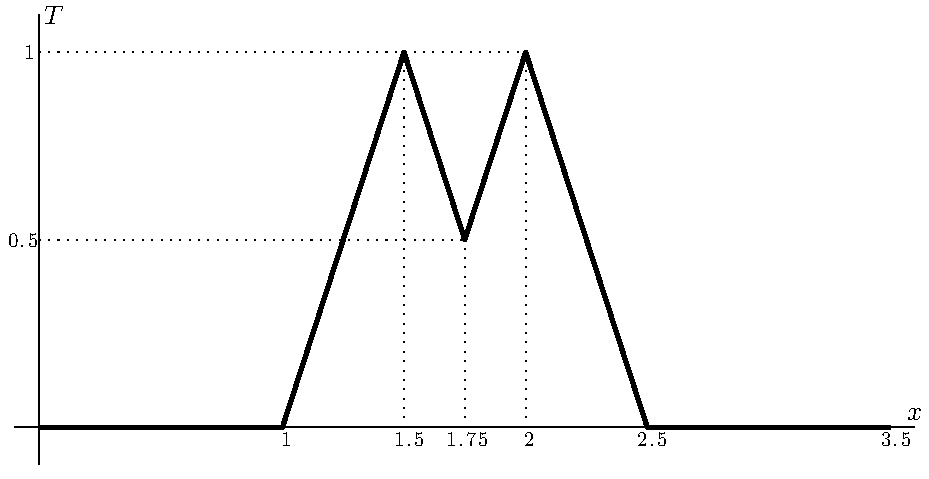
\includegraphics[width=5in]{../figs/Labs/DiffusionIC}
  \end{center}
  Overlay plots for different times on the same axis, showing the
  evolution of the temperature signal under diffusion.  Take
  $\kappa=1$.
\item Show that
  \begin{displaymath}
    \pdifftwo{\eta}{x} - \frac{1}{c^2}\pdifftwo{\eta}{t}
    = \left(\pdiff{}{x} - \frac{1}{c}\pdiff{}{t}\right)\left(\pdiff{}{x} + \frac{1}{c}\pdiff{}{t}\right)\eta.
  \end{displaymath}
\item Show that
  \begin{align}
    \pdiff{}{x} - \frac{1}{c}\pdiff{}{t} &= 2\pdiff{}{u} &\text{and}& 
    &\pdiff{}{x} + \frac{1}{c}\pdiff{}{t} &= 2\pdiff{}{v}, \nonumber   
  \end{align}
  where $u=x-ct$ and $v=x+ct$.
\item Show that $\eta(x,t) = f_1(x-ct) + f_2(x+ct)$ is a solution to
  the wave equation for a stretched string.
\item By considering two functions of your choice at times $t_1$ and
  $t_2$, show that $\eta(x,t) = f_1(x-ct)$ represents a wave
  travelling in the $+x$-direction, and that $\eta(x,t) = f_2(x+ct)$
  represents a wave travelling in the $-x$-direction.  Show that both
  travel with speed $c$.
\item Show that
  \begin{displaymath}
    \eta = A \sin(\kappa x)\sin(\omega t)
  \end{displaymath}
  is a solution to the wave equation for a stretched string.
\item In lecture we considered the case of the vibration of a plucked
  string, where we had $\eta_0(x)\ne0$ and $\dot{\eta}_0(x)=0$.  For
  this problem, consider a string with an initial velocity, but no
  initial displacement. In particular, $\eta_0(x)=0$ and
  \begin{displaymath}
    \dot{\eta}_0(x) =
    \begin{cases}
      \frac{2A}{l}x & \text{for $0\le x\le l/2$},\\
      \frac{2A}{l}(l-x) & \text{for $l/2 < x\le l$}.
    \end{cases}
  \end{displaymath}
  \begin{enumerate}
  \item Find an analytical expression for the displacement of the
    string as a function of space and time, $\eta(x,t)$.
  \item Compute the fundamental frequency $\omega_1$ and period of
    oscillation $T_1$, letting $l=100$, $A=1$, and $c=1$.
  \item Using \Mlab, plot your solution from (a) using the constants
    from (b) at $t = 0,\; T_1/4,\; T_1/3,$ and $T_1/2$.
  \end{enumerate}
\item Using the \Mlab function \texttt{dfs\_stringwaves}, plot the
  evolution of an initial condition of your choice at representative
  times including $t=0,\; T_1/4,\; T_1/3,\; T_1/2,$ and $T_1$, where
  $T_1$ is the fundamental period of the string.  Your initial
  condition must NOT be $\eta_0(x) = \sin\frac{\pi x}{l}$ (it must be
  something more complicated).  Note that the initial condition must
  respect the boundary conditions at the ends of the string.
\item \textbf{[bonus for the keen]} The function
  \texttt{dfs\_stringwaves} computes the evolution of the string's
  displacement after some initial displacement $\eta_0(x)$ but with
  zero initial velocity $\dot{\eta}_0(x)$.  In general, a string could
  vibrate due to a combination of an initial displacement and an
  initial velocity.  Extend the function \texttt{dfs\_stringwaves} to
  accommodate this generalisation.  Your new function should have the
  interface
  \begin{center}
    \texttt{function eta = dfs\_stringwaves(x,eta0,eta0dot,c,time)}
  \end{center}
  where \texttt{eta0dot} is a vector of initial speeds corresponding
  to $\dot{\eta}_0$. Verify your function against your answer to
  question 1, and then apply it to an initial condition that combines
  some nonzero $\eta_0$ and $\dot{\eta}_0$ of your choice.
\end{enumerate}

\end{document}
